% ============================================================
% 4. METHOD: DIAL
% ============================================================
\begin{figure*}[t]
	\centering
	% 请将最终导出的图片命名为 dial_pipeline.pdf 或 .png 放在项目根目录
	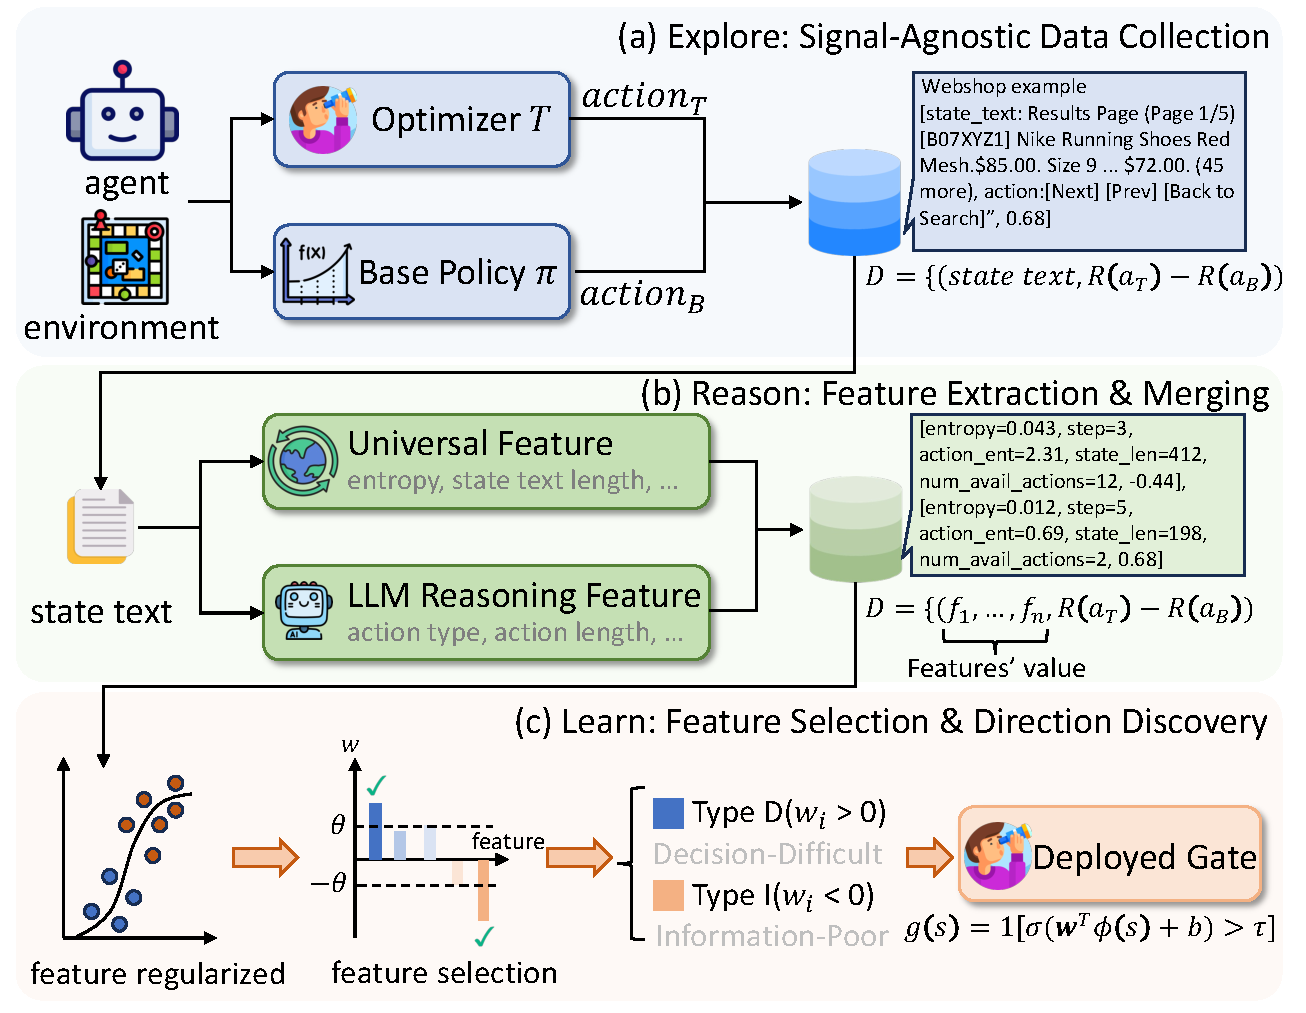
\includegraphics[width=\textwidth]{figures/dial_pipeline.pdf} 
	\caption{\textbf{The DIAL pipeline.}
		\textbf{(a) Explore}: collect signal-agnostic $(s, U)$ pairs via Bernoulli-$\varepsilon$ rollouts.
		\textbf{(b) Reason}: build a candidate feature pool $\phi(s)$ from universal metrics plus optional LLM-proposed task-specific features.
		\textbf{(c) Learn}: fit an $\ell_1$-regularized logistic gate, whose signed weights jointly perform feature selection and recover per-environment direction (Type~D: $w_i{>}0$; Type~I: $w_i{<}0$).}
	\label{fig:method_overview}
\end{figure*}
\section{Direction-Informed Adaptive Learning}
\label{sec:method}

Section~\ref{sec:signal-landscape} establishes that the
uncertainty signal $\sigma$ alone is not a sufficient statistic
for the value of computation, so any cross-setting adaptive
gate must condition on auxiliary features
$\phi(s)$ that carry information about the latent
state type $\tau(s)$. Concretely, this implies three method
constraints: per-(environment, backbone) direction discovery
(\S\ref{sec:empirical-landscape}), a multi-signal feature pool
that approximates $\tau$ (\S\ref{sec:empirical-landscape}), and
\emph{signal-agnostic} exploration---developed below---since
conditioning data collection on the very signal whose direction
is unknown introduces a self-confirming bias.

DIAL is the minimal procedure that lifts $\sigma$ toward
sufficiency for $\mathrm{VOC}$ under these constraints
(Fig.~\ref{fig:method_overview}): randomized exploration
(\S\ref{sec:explore}) collects an unbiased $(s, U)$ dataset, an
optional LLM feature layer (\S\ref{sec:reason}) extends the
universal feature pool when needed, and a sparse linear gate
(\S\ref{sec:learn}) selects which features carry information
about $\tau$ in each (environment, backbone) setting. The
sophistication of the classifier is not the contribution; the
contribution is the demonstration that once $\sigma$ is
augmented with the right auxiliary features, the simplest
possible classifier already outperforms every fixed-direction
baseline (\S\ref{sec:experiments}).

\subsection{Explore: Signal-Agnostic Data Collection}
\label{sec:explore}

Exploration collects the $(s, U)$ pairs that will be used to fit
the gate. The central constraint is signal-agnosticity: the
collection policy must not condition on any signal whose
semantics we are trying to learn. Although uncertainty-conditioned
data collection is the default in prior adaptive-gating work, it
is incompatible with the goal of \emph{learning} direction: a
gate trained on uncertainty-triggered states systematically
under-samples exactly the states that determine $\rho$'s sign,
biasing the fitted direction toward the prior assumption rather
than testing it. DIAL therefore uses the simplest policy
consistent with signal-agnosticity. At each step~$t$ in
episode~$i$, a uniform random coin flip
$z_t^{(i)} \sim \mathrm{Bernoulli}(\varepsilon_{\text{explore}})$
determines whether to trigger the optimizer~$T$ ($z_t{=}1$) or
use the base action ($z_t{=}0$). Aggregating across
$N_{\text{explore}}$ episodes yields an unbiased dataset:
\begin{equation}
  \mathcal{D} = \bigl\{
    \bigl(\phi(s_t^{(i)}),\; U_t^{(i)}\bigr)
    : z_t^{(i)} = 1
  \bigr\}_{t, i},
  \label{eq:dataset}
\end{equation}
where $U_t^{(i)} \in \{0, 1\}$ indicates whether the optimizer
improved the outcome at step~$t$, and $\phi(s)$ is the feature
vector described in \S\ref{sec:reason}.

\subsection{Reason: LLM Feature Layer}
\label{sec:reason}

The next step builds the feature pool $\phi_{\text{cand}}(s)$
that the gate will be fit over. This pool must be rich enough to
include each environment's relevant signals, but not so
environment-specific that deployment requires manual engineering
per task.
DIAL's default is a fixed set of universal features:
\texttt{step\_count}, \texttt{token\_entropy},
\texttt{state\_length}, \texttt{action\_entropy}, and others.
These are available in every environment without task-specific
engineering. In the environments we study, this pool alone is
sufficient to recover a gate that outperforms all fixed-direction
baselines (\S\ref{sec:ablation}).

For environments where universal features may be inadequate,
such as WebShop, whose gating benefits from task-specific
signals like \texttt{num\_available\_actions}, DIAL offers an
\emph{optional} automation layer: an LLM is given a summary of
$\mathcal{D}$ and proposes task-specific feature hypotheses
$\phi_{\text{LLM}}(s)$, which join the universal pool to form
$\phi_{\text{cand}}(s) = \phi_{\text{univ}}(s) \cup \phi_{\text{LLM}}(s)$.
Details of the LLM input format and prompt template are in
Appendix~\ref{app:llm-feature-layer}.
The ablation in \S\ref{sec:ablation} shows that this layer is
load-bearing only on FEVER ($+9.1$\,pp); on every other
environment its contribution is ${\leq}1.8$\,pp, and on APPS and
Plancraft it is effectively zero. We therefore present the LLM
layer as an honest extensibility mechanism rather than a core
component, and report all main-result numbers without claiming
its contribution is general.

\subsection{Learn: Sparse Linear Gate}
\label{sec:learn}

Given $\mathcal{D}$ and $\phi_{\text{cand}}$, DIAL fits an
$\ell_1$-regularized logistic regression:
\begin{equation}
\begin{aligned}
\mathbf{w}^*, b^* = \argmin_{\mathbf{w}, b}\ 
&\sum_{(\phi, U) \in \mathcal{D}}
\ell\bigl(\sigma(\mathbf{w}^\top \phi + b),\, U\bigr)\\
&+ \lambda \|\mathbf{w}\|_1
\end{aligned}
\label{eq:lasso}
\end{equation}
where $\ell$ is the binary cross-entropy loss and
$\lambda$ controls sparsity over $\phi_{\text{cand}}$ so that
uninformative features drop out. The deployed gate is
\begin{equation}
  g(s) = \mathbf{1}\!\left[\sigma(\mathbf{w}^{*\top} \phi(s) + b^*)
  > \tau\right],
  \label{eq:gate}
\end{equation}
with threshold $\tau$ set by cross-validation on $\mathcal{D}$.

\paragraph{Cost accounting.}
DIAL incurs three costs: (i)~a one-time exploration cost of
$N_{\text{explore}}{=}50$ episodes per (environment, backbone)
pair, amortized over all subsequent deployment;
(ii)~sub-second offline gate-fitting time, dominated by feature
extraction; and (iii)~per-step inference cost equal to evaluating
$\phi(s)$ and a single sigmoid. Only (iii) is incurred at
deployment, and it is zero relative to a non-gated agent: there
is no extra LLM call, no $K$-way voting, and no calibration
query. Implementation details are in
Appendix~\ref{app:dial-details}.

\paragraph{Signed weights as a diagnostic.}
The $\ell_1$ penalty in Eq.~\ref{eq:lasso} simultaneously
performs feature selection and direction discovery. The sign of
each fitted weight provides an interpretable per-environment
estimate of the Two-Source mixture of \S\ref{sec:toy-model}:
$w_i > 0$ indicates the environment sits on the Type~D side of
the reversal threshold $p_I^*$ for signal~$i$ (high signal
$\to$ trigger), $w_i < 0$ the Type~I side (high signal $\to$
\emph{don't} trigger), and $w_i \approx 0$ an uninformative
signal. The complete pipeline, including online adaptation for
drifting environments, is summarized in
Algorithm~\ref{alg:dial} (Appendix~\ref{app:dial-details}).